\documentclass{article}\usepackage[]{graphicx}\usepackage[]{color}
% maxwidth is the original width if it is less than linewidth
% otherwise use linewidth (to make sure the graphics do not exceed the margin)
\makeatletter
\def\maxwidth{ %
  \ifdim\Gin@nat@width>\linewidth
    \linewidth
  \else
    \Gin@nat@width
  \fi
}
\makeatother

\definecolor{fgcolor}{rgb}{0.345, 0.345, 0.345}
\newcommand{\hlnum}[1]{\textcolor[rgb]{0.686,0.059,0.569}{#1}}%
\newcommand{\hlstr}[1]{\textcolor[rgb]{0.192,0.494,0.8}{#1}}%
\newcommand{\hlcom}[1]{\textcolor[rgb]{0.678,0.584,0.686}{\textit{#1}}}%
\newcommand{\hlopt}[1]{\textcolor[rgb]{0,0,0}{#1}}%
\newcommand{\hlstd}[1]{\textcolor[rgb]{0.345,0.345,0.345}{#1}}%
\newcommand{\hlkwa}[1]{\textcolor[rgb]{0.161,0.373,0.58}{\textbf{#1}}}%
\newcommand{\hlkwb}[1]{\textcolor[rgb]{0.69,0.353,0.396}{#1}}%
\newcommand{\hlkwc}[1]{\textcolor[rgb]{0.333,0.667,0.333}{#1}}%
\newcommand{\hlkwd}[1]{\textcolor[rgb]{0.737,0.353,0.396}{\textbf{#1}}}%
\let\hlipl\hlkwb

\usepackage{framed}
\makeatletter
\newenvironment{kframe}{%
 \def\at@end@of@kframe{}%
 \ifinner\ifhmode%
  \def\at@end@of@kframe{\end{minipage}}%
  \begin{minipage}{\columnwidth}%
 \fi\fi%
 \def\FrameCommand##1{\hskip\@totalleftmargin \hskip-\fboxsep
 \colorbox{shadecolor}{##1}\hskip-\fboxsep
     % There is no \\@totalrightmargin, so:
     \hskip-\linewidth \hskip-\@totalleftmargin \hskip\columnwidth}%
 \MakeFramed {\advance\hsize-\width
   \@totalleftmargin\z@ \linewidth\hsize
   \@setminipage}}%
 {\par\unskip\endMakeFramed%
 \at@end@of@kframe}
\makeatother

\definecolor{shadecolor}{rgb}{.97, .97, .97}
\definecolor{messagecolor}{rgb}{0, 0, 0}
\definecolor{warningcolor}{rgb}{1, 0, 1}
\definecolor{errorcolor}{rgb}{1, 0, 0}
\newenvironment{knitrout}{}{} % an empty environment to be redefined in TeX

\usepackage{alltt}

\title{Dados orçamentários dos estados na Matriz de Saldos Contábeis (MSC)}
\author{Gabriel Junqueira}
\date{Junho de 2021}
\IfFileExists{upquote.sty}{\usepackage{upquote}}{}
\begin{document}

\maketitle

\textbf{}





\begin{tabular}{r|l|l|r|r|r|r|r}
\hline
cod\_ibge & ente & regiao & exercicio & populacao & pop\_perc & pop\_acum & posicao\\
\hline
35 & São Paulo & SE & 2021 & 46289333 & 0.2185978 & 0.2185978 & 1\\
\hline
31 & Minas Gerais & SE & 2021 & 21292666 & 0.1005530 & 0.3191508 & 2\\
\hline
33 & Rio de Janeiro & SE & 2021 & 17366189 & 0.0820105 & 0.4011613 & 3\\
\hline
29 & Bahia & NE & 2021 & 14930634 & 0.0705088 & 0.4716701 & 4\\
\hline
41 & Paraná & SU & 2021 & 11516840 & 0.0543874 & 0.5260575 & 5\\
\hline
43 & Rio Grande do Sul & SU & 2021 & 11422973 & 0.0539441 & 0.5800016 & 6\\
\hline
26 & Pernambuco & NE & 2021 & 9616621 & 0.0454138 & 0.6254153 & 7\\
\hline
23 & Ceará & NE & 2021 & 9187103 & 0.0433854 & 0.6688007 & 8\\
\hline
15 & Pará & NO & 2021 & 8690745 & 0.0410414 & 0.7098421 & 9\\
\hline
42 & Santa Catarina & SU & 2021 & 7252502 & 0.0342494 & 0.7440915 & 10\\
\hline
\end{tabular}



\begin{knitrout}
\definecolor{shadecolor}{rgb}{0.969, 0.969, 0.969}\color{fgcolor}\begin{figure}
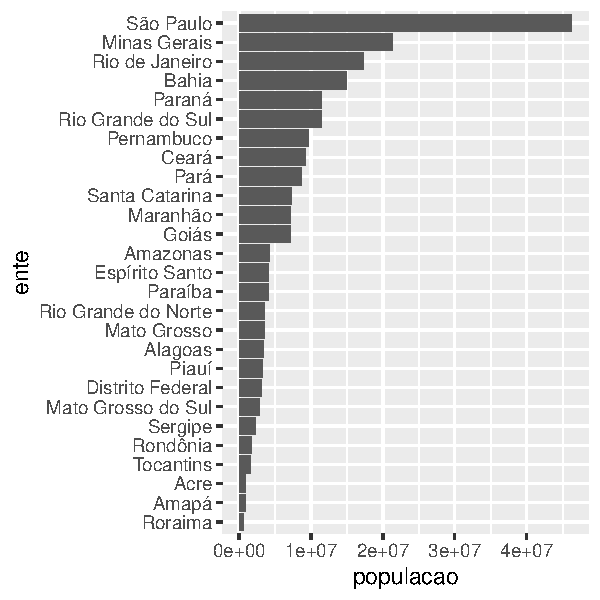
\includegraphics[width=\maxwidth]{figure/unnamed-chunk-3-1} \caption[Titulo de Figura]{Titulo de Figura}\label{fig:unnamed-chunk-3}
\end{figure}

\end{knitrout}



\end{document}
